\documentclass[12pt]{article}

\usepackage{graphicx}
\usepackage[margin=1.0in]{geometry}
\usepackage{amsmath}
\usepackage{cases}
\usepackage{amsfonts}
\usepackage{amssymb}
\usepackage{grffile}
\usepackage{setspace}

\setlength\parindent{0pt}

\author{Xiaohui Chen \\EID: xc2388}
\title{M 362K Post-Class Homework 12}


\begin{document}
\maketitle
\begin{spacing}{2.0}

\section*{5-1}

\subsection*{(a)}

\begin{figure}
\centering
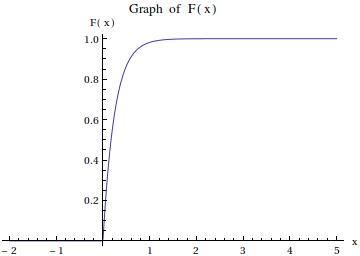
\includegraphics[width=4in]{out1}

\caption{Plot of $F(x)$}
\label{out1}

\end{figure}

The Plot is shown in Figure \ref{out1}

(a) From the plot, we can know that $F(x)$ is a non-decreasing function

(b) $\lim\limits_{x\rightarrow -\infty} F(x) = 0$

(c) $\lim\limits_{x\rightarrow \infty} F(x) = 1$

Therefore $F(x)$ has the properties of a cumulative distribution function

\subsection*{(b)}

We know that $f(x)=F'(x)$

Therefore,

\begin{numcases}{f(x)}
0 & if $x<0$\\
4e^{-4x} & if $x>0$\\
undefined & if $x=0$
\end{numcases}

\subsection*{(c)}

Distribution function:

$Pr(1 < x \le 2)= F(2)-F(1)= 1-e^{-8}-1+e^{-4}\approx 0.0179802 $

Density function:

$Pr(1 < x \le 2)= \int_{1}^{2} f(x) dx = \int_{1}^{2} 4e^{-4x} dx = 0.0179802$

\subsection*{(d)}

$Pr[X>2|X>1]= \frac{Pr[X>2 \cap X>1]}{Pr[X>1]}= \frac{Pr[X>2]}{Pr[X>1]}= \frac{1-F(x=2)}{1-F(x=1)}= \frac{e^{-8}}{e^{-4}}= 0.0183156 $

\section*{5-3}

\subsection*{(a)}

In order to have a valid density funtion, $\int_{0}^{\infty} f(y)=1$ must be true

$\int_{0}^{\infty} ke^{-3y}= \frac{k}{3}=1$

$\therefore k=3$

\subsection*{(b)}

From the density function we can know that the CDF is 

$F(y)= \int_{0}^{y} ke^{-3y} dy= -\frac{1}{3} ke^{-3y}+\frac{k}{3}$

$Therefore F(\infty)= \frac{k}{3}=1$

Therefore $k=3$

\subsection*{(c)}

From part (b) we know that the CDF is:

\begin{numcases}{F(y)=}
-e^{-3y}+1 & if $y\ge 0$\\
0 & if $y < 0$
\end{numcases}

CDF:

$Pr(2 < y \le 3)= F(3)-F(2)= -e^{-9}+e^{-6}= 0.00235534$

Density function:

$Pr(2 < y \le 3)= \int_{2}^{3} 3e^{-3y} dy = 0.00235534$

\subsection*{(d)}

$Pr(Y > -3)= F(\infty)- F(-3)= 1$

\section*{5-5}

$Pr(x<2|x\ge 1.5)= \frac{Pr( 1.5 \le x < 2 )}{Pr(x \ge 1.5)}= \frac{\int_{1.5}^2 3x^{-4} dx}{ 1-\int_{1}^{1.5} 3x^{-4} dx}= 0.578125$

Therefore the answer is (A)

\section*{5-7}

$Pr(x<5)= \int_{0}^{5} (10+x)^{-2} dx = \frac{1}{30}= 0.0333$

Therefore the answer is (A)

\end{spacing}
\end{document}
